\subsection{Dynamic Features}

Supervectors don't include information about the dynamics of the MFCCs over time. Even though
the acoustic features do include deltas and double-deltas, these features only relates the
information of adjacent frames.

The evolution of the MFCCs over time can be modeled by using different interpolation techniques,
and Dynamic Features are obtained by extracting the coefficients of the interpolation functions.
Given a phone instance,
the values of each of the MFCCs, deltas and double-deltas along the whole interval are
interpolated separately, so a total of 39 functions are computed.
The chosen methods for the current work are Legendre Polynomials and Discrete Cosine Transform.

The important thing about Dynamic Features is that they
may carry information complementary to supervectors' information, that can be used to improve
the performance of the SVM classifier. A potential gain in the combination
of Supervectors with Dynamic Features is therefore an interesting
subject to be studied and it is the main topic of the current thesis.

\subsection{Legendre}

Legendre polynomials are frequently encountered in physics and engineering.
For example, Legendre is widely used in the determination of wave
functions of electrons in the orbits of an atom, or in the determination of potential
functions in the spherically symmetric geometry \cite{legendre_usage}.
With regard to speech processing,
this technique has been used successfully
in the speaker recognition field \cite{legendre}.

\textit{Legendre functions} are the solutions to \textit{Legendre's differential equation}:

\begin{equation}
(1-x^{2})y''(x)-2xy'(x)+n(n+1)y(x)=0, \ for -1 \leq x \leq 1
\end{equation}

The solution for each particular $n={0, 1, 2 \dotsc} \in \mathbb{N}$ is a polynomial of degree
$n$: $P_{n}(x)$. These solutions are well known for each $n \in \mathbb{N}$, and they can even
be generated recursively. The first five Legendre Polynomials (Fig. \ref{fig:legendre_base}) are:

\begin{itemize}
  \label{itemize:legendreTerms}
  \item[] $P_{0}(x) = 1$
  \item[] $P_{1}(x) = x$
  \item[] $P_{2}(x) = \frac{1}{2}(3x^{2} - 1)$
  \item[] $P_{3}(x) = \frac{1}{2}(5x^{3} - 3x)$
  \item[] $P_{4}(x) = \frac{1}{8}(35x^{4} - 30x^{2} + 3)$
\end{itemize}

\begin{figure}[H]
  \centering
  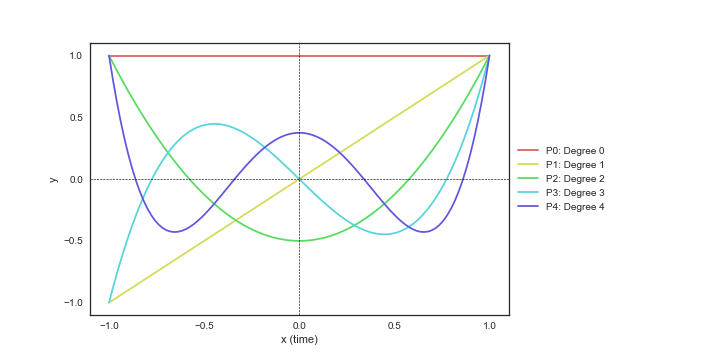
\includegraphics[width=0.75\textwidth]{files/figures/method/legendre_base}
  \centering
  \caption{First five Legendre Polynomials in the \\ interval [-1, 1]}
  \label{fig:legendre_base}
\end{figure}

Legendre Polynomials are orthogonal with respect to the $L2 \ norm$ on the interval \mbox{$-1 \leq x \leq 1$}:

\begin{equation}
\int_{-1}^{1} P_{n}(x)*P_{m}(x)dx = 0, \ m \neq n
\end{equation}

Moreover, in the interval \mbox{$-1 \leq x \leq 1$} any function $f$ can be represented as sum of
Legendre Polynomials, leading to the Fourier-Legendre Series:

\begin{equation}
f(x) = \sum_{0}^{\infty}a_{n}P_{n}(x)
\end{equation}

An infinite terms of Legendre Polynomials over the interval \mbox{$-1 \leq x \leq 1$} can be used
to approximate any function. Each coefficient models a particular aspect of the curve: $a_{0}$
is the \textit{mean} of the segment, $a_{1}$ is the slope, $a_{2}$ gives
information about the curvature of the segment and the subsequent
coefficients model the finer details.

% \subsubsection{Lasso Regression}
Given the time instants $X=[x_{1}, x_{2} \dotsc x_{t}]$ and their respective values of a particular
MFCC coefficient at those instants: $Y=[y_{1}, y_{2} \dotsc y_{t}]$,
the problem of finding the coefficients of \textit{Legendre Polynomial} of degree $k$
(for a previously defined $k$) that best approximates
the values can be formulated in terms of a \textit{Least Squares} minimization problem:

\begin{equation}
  \min_{C} {\| AC - Y \|}^{2}
\end{equation}

where the solution of the system $C$ is a ($k+1$) vector that represents the coefficients
of the \textit{Legendre Polynomial} of degree $k$ that best approximates the curve.
$A$ is a $t$ x ($k$+1) matrix, where each column $i$ represents the result of computing
\textit{Legendre's} $P_{i}$ polynomial (\ref{itemize:legendreTerms}) for each of the values
$[x_{1}, x_{2}, \dotsc x_{t}]$, also known as the \textit{Legendre-Vandermonde} matrix:

\begin{equation}
  A =
    \begin{pmatrix}
      P_{0}(x_{1}) & P_{1}(x_{1}) & \cdots & P_{k}(x_{1}) \\
      P_{0}(x_{2}) & P_{1}(x_{2}) & \cdots & P_{k}(x_{2}) \\
      \vdots & \vdots & \ddots & \vdots \\
      P_{0}(x_{t}) & P_{1}(x_{t}) & \cdots & P_{k}(x_{t}) \\
    \end{pmatrix}
\end{equation}

When modeling a particular event is preferable to pick the simplest hypothesis that best
explains the observations, because simpler hypothesis usually generalize better to new
observations than more complex hypotheses. As it was said before, the higher the
degree of the \textit{Legendre Polynomial},
the more subtle details it models. In order to achieve the right balance between decreasing
the least squares error and keeping the hypothesis simple two different approaches are taken.
On the one hand the degree of the polynomial $k$ is limited up to a few coefficients.
On the other hand, a regularization technique of the \textit{Least Squares} family's
problems is applied.

\subsubsection{Lasso Regression}

A regularization technique is evaluated along with the Legendre Polynomials. Its name is
\textit{Lasso Regression} and it modifies the
% The chosen regularization technique is called \textit{Lasso Regression}, and it modifies the
original minimization problem by adding an additional term that penalizes the L1 norm of the
solution:

\begin{equation}
  \min_{C} {\| AC - Y \|}^{2} + \lambda \| C \|_{1}
\end{equation}

Regularization terms leads to solutions where more responsibility is assigned to the
coefficients that contributes the most in lowering the error term while
shrinking the coefficients with less contribution to lowering the error.

There exists other alternatives to \textit{Lasso} with regard to regularization.
A widely-used one is \textit{Tikhonov Regularization}, also known as \textit{Ridge Regression},
where the square of the \textit{L2 norm} ($\| C \|_{2}^{2}$) is used as regularization term.

Unlike the square of the \textit{L2 norm},
the \textit{L1 norm} ($\| C \|_{1}$)
% instead of the standard
% square of the \textit{L2 norm} ($\| C \|_{2}^{2}$)
leads to an interesting and useful property:
In \textit{Ridge Regression}, as the penalty is increased, all parameters are reduced while
still remaining non-zero, while in \textit{Lasso} increasing the penalty will cause more and
more of the parameters to be driven to zero. Thus \textit{Lasso} automatically selects more
relevant features and discards the others whereas \textit{Ridge Regression} never fully
discards any features.


\subsection{Discrete Cosine Transform}

An alternative to Legendre Polynomials to capture the general aspects of the utterance in order to
summarize the information carried out by the \textit{MFCCs} across time is the
\textit{Discrete Cosine Transform}. Variations on the values of MFCCs through time may be
better explained
using periodic functions instead of polynomial ones for some phones,
making \textit{DCT} a more suitable technique
for those phones. \textit{DCT} is used in many processes related with science and engineering
such as lossy compression of audio (e.g. \textit{MP3}) and images (e.g. \textit{JPEG}), which are
among the most popular formats in their respective fields. This technique has also been used
to approximate prosodic features in speaker verification tasks \cite{dct}.

\textit{DCT} belongs to the family of the Fourier analysis. As a member of the family, it
provides a way to approximate a general function by sums of simpler trigonometric functions.
These transformations map a function to a set of coefficient of basis functions, where
the basis functions are sinusoidal and are therefore strongly localized in the frecuency spectrum.
In particular, \textit{DCT} expresses a finite sequence of data points in terms of a sum of
\textit{cosine} functions oscillating at different frequencies. Unlike the
\textit{Fourier Transform} that expresses the sequence in terms of both sine and cosine functions,
thus needing a complex number to represent the coefficient of each frecuency, it only uses real
numbers to output the coefficient of each frecuency.

There exists different variants of the \textit{DCT}, being the type-II
the most common and the one that it is used in the current work:

\begin{equation}
X_{k} = \sum_{n=0}^{N-1} x_{n} cos \Big[ \frac{\pi}{N} \Big( n + \frac{1}{2} \Big) k \Big], \ for \ k = [0, 1, \dotsc, N-1]
\end{equation}

where $N$ is the number of the extracted samples of the signal to be decomposed.
In this way, $n$ coefficients are obtained corresponding to each of the frequencies from
$0$ to $N-1$. An illustration of the curves with the first two frequencies is shown in
Fig. \ref{fig:dct_base}. Each coefficient is obtained from the sum of the individual contributions
of the samples to the $k^{th}$ frequency.

\begin{figure}[H]
  \centering
  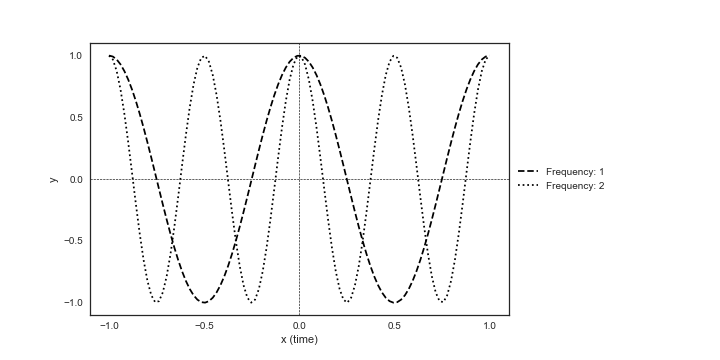
\includegraphics[width=0.75\textwidth]{files/figures/method/dct_base}
  \centering
  \caption{Basis cosine functions of frequencies 1 and 2 over the interval [-1, 1]}
  \label{fig:dct_base}
\end{figure}

As in Legendre Polynomials,
the number of coefficients to be obtained is again limited up to a few coefficients to
avoid overfitting to the training set. However, unlike Legendre where it is possible to
specify as an input parameter the number of coefficients to be used when computing the polynomial,
the DCT does not have such option. Given a set of $n$ points, DCT
always computes $n$ coefficients, so when extracting the features for the SVM classifier only
the first $k$ coefficients are extracted, while the other ones are discarded.

\subsection{Comparison between Legendre and DCT}

To conclude this section an illustrative visual example that compares the approximations made
by both techniques for a given set of values is included in Fig. \ref{fig:dynamic_features_comparison}. The values are extracted from
the 4\textsuperscript{th} MFCC of an instance of the phone 'i', taken from the training set.

\begin{figure}[H]
  \centering
  \begin{subfigure}{.5\textwidth}
    \centering
    \captionsetup{width=.95\linewidth}
    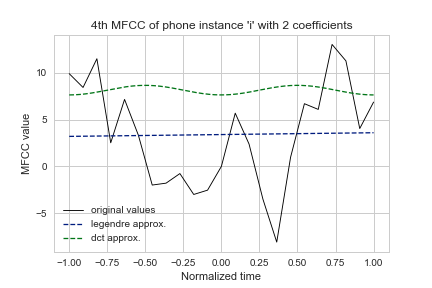
\includegraphics[width=.95\linewidth]{files/figures/method/dynamic_features_2}
    \caption{Approximations of Legendre Polynomials with 2 coefficients (degree 1),
    and DCT with 2 coefficients.}
    \label{fig:dynamic_features_1}
  \end{subfigure}%
  \begin{subfigure}{.5\textwidth}
    \centering
    \captionsetup{width=.95\linewidth}
    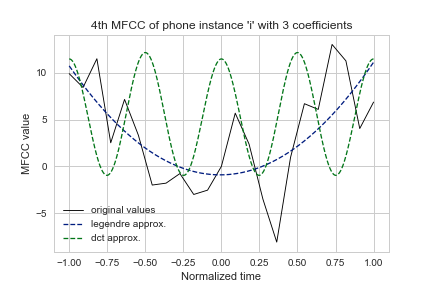
\includegraphics[width=.95\linewidth]{files/figures/method/dynamic_features_3}
    \caption{Approximations of Legendre Polynomials with 3 coefficients (degree 2),
    and DCT with 3 coefficients.}
    \label{fig:sub2}
  \end{subfigure}
  \caption{}
  \label{fig:dynamic_features_comparison}
\end{figure}

\begin{figure}[H]
  \centering
  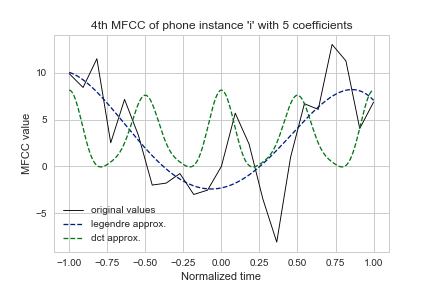
\includegraphics[width=0.5\textwidth]{files/figures/method/dynamic_features_5}
  \caption{Approximation of Legendre Polynomials with 5 coefficients (degree 4),
    and DCT with 5 coefficients.}
\end{figure}

Legendre Polynomials are better at capturing the overall shape of the curve while DCT
is better at modeling the oscilations of the curve. Comparative experiments are carried
out in this work
in order to find which is the dynamic feature that best complements the supervectors when
training the SVM classifier.

